\documentclass[../teoria.root.tex]{subfiles}

\begin{document}

\section{Rectas}

\subsection{En el origen}

Una recta es simplemente un conjunto de vectores que, bueno, tienen la forma de
una recta. En una recta que pasa por el origen, todos los vectores son
paralelos, asi que dado un vector $\vec{v}$, una recta que pasa por el origen
con direccion $\vec{v}$ seria
$\mathbb{L}=\{X\in\mathbb{R}^2:X=k\vec{v},k\in\mathbb{R}\}$, el conjunto de
todos los vectores multiplos, y por lo tanto paralelos, de $\vec{v}$.

\begin{center}
	\begin{tikzpicture}
		\draw[help lines] (-3,-2) grid(5,3);
		\draw[->] (-3,0) -- (5,0) node[right]{$x$};
		\draw[->] (0,-2) -- (0,3) node[above]{$y$};
		\coordinate (v) at (2,1);
		\foreach \k in {-2,-1,2,3} {
			\draw[->,red,thick] (0,0) -- ($\k*(v)$) node[pos=1,sloped,above]{$\k\vec{v}$};
		}
		\draw[->,green,very thick] (0,0) -- (v) node[pos=1,sloped,above]{$\vec{v}$};
	\end{tikzpicture}
\end{center}

\subsection{Pasando por un punto}

Para describir rectas que no pasan por el origen, lo unico que se necesita
hacer es conseguir un punto que pertenezca a la recta, y sumarselo a la cuenta
anterior. Una recta que pasa por el punto $P$ con direccion $\vec{v}$ seria
$\mathbb{L}=\{X\in\mathbb{R}^2:X=k\vec{v}+P,k\in\mathbb{R}\}$:

\begin{center}
	\begin{tikzpicture}
		\draw[help lines] (-3,-2) grid(5,3);
		\draw[->] (-3,0) -- (5,0) node[right]{$x$};
		\draw[->] (0,-2) -- (0,3) node[above]{$y$};
		\coordinate (v) at (2,1);
		\coordinate (p) at (-1,2);
		\foreach \k in {-2,-1,1,2,3} {
			\coordinate (o) at ($\k*(v)$);
			\coordinate (l) at ($\k*(v)+(p)$);
			\draw[->,help lines,thick] (0,0) -- (o);
			\draw[help lines,dashed] (o) -- (l);
			\draw[->,red,thick] (0,0) -- (l) node[rotate=30,above]{$\k\vec{v}+P$};
			\draw[purple,thick] (p) -- (l);
		}
		\draw[->,green,very thick] (0,0) -- (v) node[pos=1,sloped,above]{$\vec{v}$};
		\draw[->,blue,very thick] (0,0) -- (p) node[rotate=30,above]{$P$};
	\end{tikzpicture}
\end{center}

\subsection{Ecuación paramétrica}

Usar la notación de conjuntos para definir una recta es bastante incomodo, así
que de ahora en adelante vamos a usar lo que se conoce como la ecuación
paramétrica de la recta. La ecuación paramétrica de una recta $\mathbb{L}$ que
pasa por $P$ en la dirección de $\vec{v}$ se escribe:
\[\mathbb{L}:X=\lambda\vec{v}+P\]

La letra $\lambda$ no representa una constante, sino que seria una variable que
se reemplaza por cualquier numero real. $\vec{v}$ seria el \textit{vector
director} de la recta, y $P$ seria el \textit{punto de paso}. Cabe aclarar que
distintas ecuaciones paramétricas pueden representar la misma recta, ya que
cualquier vector paralelo a la recta se puede usar como director, y cualquier
vector en la recta se puede usar como punto de paso.

\subsection{Pasando por dos puntos}

Dados dos puntos $A$ y $B$, encontrar la recta que pasa por ambos puntos es
bastante fácil. Cualquiera de los puntos nos sirve como el punto de paso, y un
vector director se puede conseguir usando el vector $\vec{AB}$, que si
recuerdan de la sección anterior, se consigue haciendo $B-A$.
\[\mathbb{L}:X=\lambda(B-A)+A\]

\begin{center}
	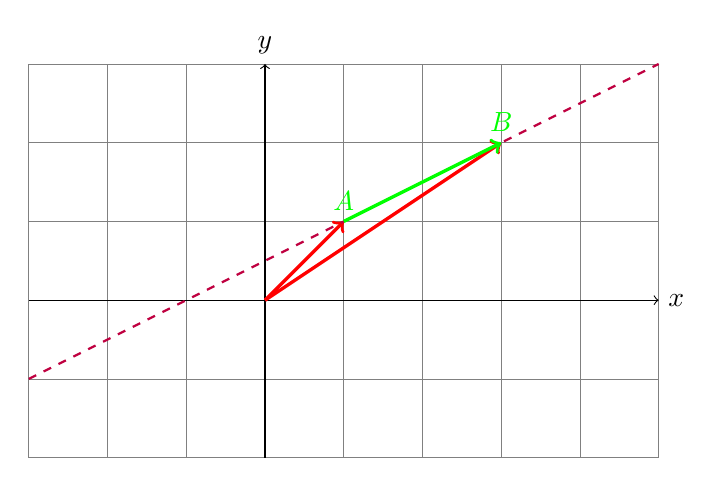
\begin{tikzpicture}
		\draw[help lines] (-3,-2) grid(5,3);
		\draw[->] (-3,0) -- (5,0) node[right]{$x$};
		\draw[->] (0,-2) -- (0,3) node[above]{$y$};
		\coordinate (a) at (1,1);
		\coordinate (b) at (3,2);
		\draw[->,red,very thick] (0,0) -- (a) node[green,above]{$A$};
		\draw[->,red,very thick] (0,0) -- (b) node[green,above]{$B$};
		\draw[dashed,purple,thick] (-3,-1) -- (5,3);
		\draw[->,green,very thick] (a) -- (b);
	\end{tikzpicture}
\end{center}

\subsection{Pertenencia de punto a recta}

Para saber si un punto pertenece a una recta, hay que encontrar un valor
$\lambda\in\mathbb{R}$ que al ser reemplazado en la ecuación paramétrica de la
recta resulte en el punto en cuestion. Para encontrarlo tan solo hay que
reemplazar el punto en la ecuación paramétrica. Por ejemplo, para ver si el
punto $(0,7,-1)$ pertenece a la recta $\mathbb{L}:X=\lambda(2,-3,1)+(4,1,1)$:
\begin{gather*}
	\begin{split}
		\mathbb{L}:X&=\lambda(2,-3,1)+(4,1,1)\\
		(0,7,-1)\in\mathbb{L}\implies(0,7,-1)&=\lambda(2,-3,1)+(4,1,1)\\
		(0,7,-1)&=(2\lambda,-3\lambda,\lambda)+(4,1,1)\\
		(0,7,-1)&=(2\lambda+4,-3\lambda+1,\lambda+1)\\
	\end{split}\\
	\begin{cases}
		0=2\lambda+4\\
		7=-3\lambda+1\\
		-1=\lambda+1
	\end{cases}\\
	\begin{cases}
		\lambda=-2\\
		\lambda=-2\\
		\lambda=-2
	\end{cases}\\
	\begin{split}
		(0,7,-1)&=-2(2,-3,1)+(4,1,1)\\
		(0,7,-1)&=(-4,6,-2)+(4,1,1)\\
		(0,7,-1)&=(0,7,-1)
	\end{split}
\end{gather*}

Si hacemos esto con un vector que no forme parte de $\mathbb{L}$, como
$(6,-2,1)$, inevitablemente vamos a encontrarnos con una contradicción:
\begin{gather*}
	\begin{split}
		\mathbb{L}:X&=\lambda(2,-3,1)+(4,1,1)\\
		(6,-2,1)\in\mathbb{L}\implies(6,-2,1)&=\lambda(2,-3,1)+(4,1,1)\\
		(6,-2,1)&=(2\lambda,-3\lambda,\lambda)+(4,1,1)\\
		(6,-2,1)&=(2\lambda+4,-3\lambda+1,\lambda+1)
	\end{split}\\
	\begin{cases}
		6=2\lambda+4\\
		-2=-3\lambda+1\\
		1=\lambda+1
	\end{cases}\\
	\begin{cases}
		\lambda=1\\
		\lambda=1\\
		\lambda=0
	\end{cases}
\end{gather*}

\subsection{Rectas Paralelas y Perpendiculares}

Dos rectas son paralelas si sus vectores directores son paralelos. Lo mismo
pasa con rectas perpendiculares.

\begin{center}
	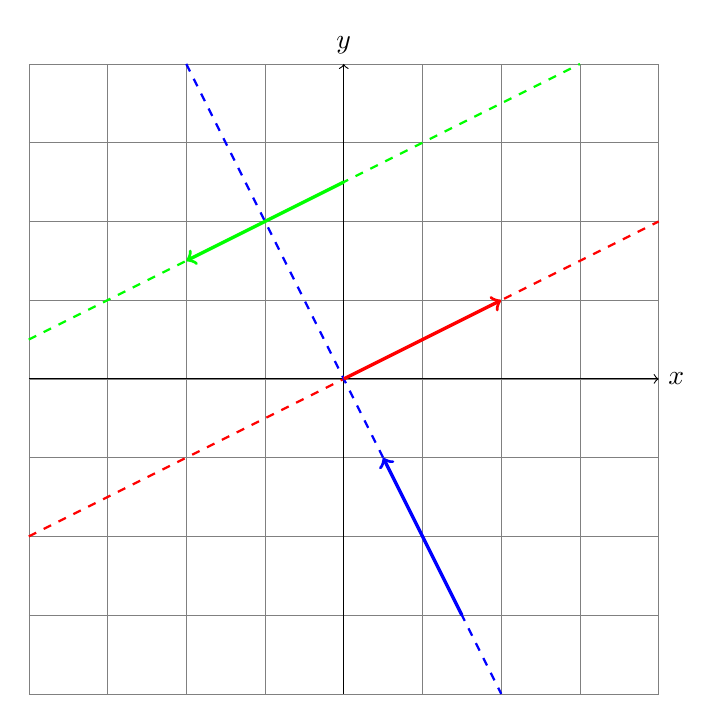
\begin{tikzpicture}
		\draw[help lines] (-4,-4) grid(4,4);
		\draw[->] (-4,0) -- (4,0) node[right]{$x$};
		\draw[->] (0,-4) -- (0,4) node[above]{$y$};
		\draw[red,dashed,thick] (-4,-2) -- (4,2);
		\draw[green,dashed,thick] (-4,.5) -- (3,4);
		\draw[blue,dashed,thick] (-2,4) -- (2,-4);
		\draw[->,red,very thick] (0,0) -- (2,1);
		\draw[->,green,very thick] (0,2.5) -- ++(-2,-1);
		\draw[->,blue,very thick] (1.5,-3) -- ++(-1,2);
	\end{tikzpicture}
\end{center}

\subsection{Ecuación Implícita en $\mathbb{R}^2$}

Existe otra manera de describir una recta en dos dimensiones: Con un punto $P$
que pase por la recta, y un vector $\vec{v}$ perpendicular a la misma. Todos
los puntos $X$ tal que el vector $\vec{PX}$ sea perpendicular a $\vec{v}$
forman parte de la recta:

\begin{center}
	\begin{tikzpicture}
		\draw[help lines] (-2,-2) grid(5,3);
		\draw[->] (-2,0) -- (5,0) node[right]{$x$};
		\draw[->] (0,-2) -- (0,3) node[above]{$y$};
		\coordinate (p) at (2,1);
		\pgfmathsetmacro{\vx}{-0.5};
		\pgfmathsetmacro{\vy}{1};
		\coordinate (v) at (\vx,\vy);
		\draw[->,red,very thick] (p) -- ++(v);
		\foreach \k in {-4,-3,-2,-1,1,2,3} {
			\draw[->,thick,purple] (p) -- ++($\k*(\vy,-\vx)$);
		};
		\fill[green] (p) circle(2pt) node[below right]{$P$};
	\end{tikzpicture}
\end{center}

Por ejemplo, para describir una recta que pasa por el punto $(1,-3)$ y tiene un
vector perpendicular $(2,3)$:
\begin{align*}
	(X-P)\perp\vec{v}\iff(X-P)\cdot\vec{v}&=0\\
	((x,y)-(1,-3))\cdot(2,3)&=0\\
	(x-1,y+3)\cdot(2,3)&=0\\
	2x-2+3y+9&=0\\
	2x+3y&=-7
\end{align*}

Esta ecuación describe a la recta de una forma distinta a la ecuación
paramétrica, y se llama la \textit{ecuación implícita} de la recta.

Si nos dan una recta $\mathbb{L}:\lambda\vec{v}+P$, se puede construir su
ecuación implícita encontrando un vector $\vec{w}\perp\vec{v}$, como
$(v_y,-v_x)$, y haciendo la ecuación $(x,y)\cdot\vec{w}=P\cdot\vec{w}$.

Para pasar de la ecuación implícita a la paramétrica, solo necesitamos
encontrar dos puntos de la recta, reemplazando $x$ o $y$ por dos valores a
nuestra elección, y despejando la coordenada restante, y luego calcular la
recta que pasa por ambos puntos.

\subsection{Intersección de rectas}

Para encontrar el conjunto $\mathbb{L}_1\cap\mathbb{L}_2$, los puntos que
forman la intersección entre las rectas, sencillamente hay que igualar sus
ecuaciones paramétricas. Por ejemplo, dadas las rectas
$\mathbb{L}_1:\lambda(2,0)+(-2,3)$ y $\mathbb{L}_2:\lambda(3,1)+(-1,1)$, su
intersección se puede calcular con el siguiente procedimiento:
\begin{gather*}
	\begin{split}
		Q\in(\mathbb{L}_1\cap\mathbb{L}_2)\iff Q\in\mathbb{L}_1\land Q\in\mathbb{L}_2
	\end{split}\\
	\intertext{(Cabe aclarar que las incógnitas de las ecuaciones son
	distintas, así que usan símbolos distintos, en vez de usar $\lambda$ para
	ambas)}
	\begin{cases}
		Q=\lambda(2,0)+(-2,3)\\
		Q=\mu(3,1)+(-1,1)
	\end{cases}\\
	\begin{split}
		\lambda(2,0)+(-2,3)&=\mu(3,1)+(-1,1)\\
		(2\lambda,0)+(-2,3)&=(3\mu,\mu)+(-1,1)\\
		(2\lambda-2,3)&=(3\mu-1,\mu+1)
	\end{split}\\
	\begin{cases}
		2\lambda-2=3\mu-1\\
		3=\mu+1
	\end{cases}\\
	\begin{cases}
		2\lambda=3\mu+1\\
		\mu=2
	\end{cases}\\
	\begin{cases}
		2\lambda=3\cdot2+1\\
		\mu=2
	\end{cases}\\
	\begin{cases}
		\lambda=\frac{7}{2}\\
		\mu=2
	\end{cases}\\
	\begin{split}
		Q=\frac{7}{2}(2,0)+(-2,3)&=2(3,1)+(-1,1)=(5,3)
	\end{split}
\end{gather*}

En el caso anterior, las rectas se tocaban únicamente en un punto, pero puede
ser que dos ecuaciones paramétricas describan la misma recta. Por ejemplo,
$\mathbb{L}_1:\lambda(2,-1)+(-2,3)$ y $\mathbb{L}_2:\lambda(-4,2)+(0,2)$:
\begin{gather*}
	\begin{split}
		\lambda(2,-1)+(-2,3)&=\mu(-4,2)+(0,2)\\
		(2\lambda,-\lambda)+(-2,3)&=(-4\mu,2\mu)+(0,2)\\
		(2\lambda-2,-\lambda+3)&=(-4\mu,2\mu+2)
	\end{split}\\
	\begin{cases}
		2\lambda-2=-4\mu\\
		-\lambda+3=2\mu+2
	\end{cases}\\
	\begin{cases}
		\lambda=-2\mu+1\\
		-\lambda+3=2\mu+2
	\end{cases}\\
	\tag{Reemplazo $\lambda$}
	\begin{cases}
		\lambda=-2\mu+1\\
		-(-2\mu+1)+3=2\mu+2
	\end{cases}\\
	\begin{cases}
		\lambda=-2\mu+1\\
		\cancel{2\mu+2}=\cancel{2\mu+2}
	\end{cases}\\
	\begin{cases}
		\lambda=-2\mu+1\\
		0=0
	\end{cases}
\end{gather*}

El sistema de ecuaciones quedo con una variable independiente, osea que para
cualquier valor de $\lambda$, existe un valor de $\mu$ valido. Por lo tanto,
todos los puntos de las rectas están en intersección, así que las rectas son
iguales:
\[\mathbb{L}_1\cap\mathbb{L}_2=\mathbb{L}_1=\mathbb{L}_2\]

Si al igualar las rectas llegáramos a encontrar a una contradicción,
significaría que las rectas nunca se tocan. En $\mathbb{R}^2$, esto solo puede
ocurrir si las rectas son paralelas, pero en $\mathbb{R}^3$ y mayores esto no
siempre es verdad.

\end{document}
